\documentclass{beamer} %a prezentációhoz
%\documentclass[handout]{beamer} % a honlapra feltöltendő verzióhoz
% \usecolortheme{beaver}
% \usetheme{Hannover}
% \usetheme{Berkeley}
% \usetheme{Goettingen}

%\useoutertheme[left]{sidebar}
%\usepackage{default}
\usepackage[magyar]{babel}

\usepackage[utf8]{inputenc}
\usepackage{amsmath, amscd}
\usepackage{amssymb}
\usepackage{enumerate}
\usepackage{graphics}
\usepackage{graphicx}
\usepackage{array}
\newcolumntype{L}[1]{>{\raggedright\let\newline\\\arraybackslash\hspace{0pt}}m{#1}}
\newcolumntype{C}[1]{>{\centering\let\newline\\\arraybackslash\hspace{0pt}}m{#1}}
\newcolumntype{R}[1]{>{\raggedleft\let\newline\\\arraybackslash\hspace{0pt}}m{#1}}

\usepackage{overpic}

\usepackage{color}
%\usepackage[usenames,dvipsnames]{pstricks}
\usepackage{epsfig}
\usepackage{tikz}
\usepackage{pgf}
\usefonttheme[onlymath]{serif}


\graphicspath{{figs/}}

\usepackage[normalem]{ulem}
\usepackage{listings}
\usepackage{color}
\definecolor{dkgreen}{rgb}{0,0.6,0}
\definecolor{gray}{rgb}{0.5,0.5,0.5}
\definecolor{mauve}{rgb}{0.58,0,0.82}
\definecolor{sideb}{rgb}{0.84,0.84,0.94}
\definecolor{lightblue}{rgb}{0.72,0.86,0.96}
\newcommand{\myemph}[1]{{\color{blue}#1}}
\frenchspacing

\title{Bevezetés a \LaTeX{} használatába 2.}
\author[Vida György]{Vida György}
\institute[WJSz]{Programozás szeminárium \\ Wigner Jenő Szakkollégium \\ BME TTK}

\date[2014.\ március 24.]{2014.\ március 24. \\[0.5cm] 
\includegraphics[width=0.27\paperwidth]{bme_logo_kicsi}\hspace{0.27cm}
\includegraphics[height=1.7cm]{WJSz_logo_black}}

%\pgfdeclareimage[height=2.25ex,width=2.5\baselineskip]{BME}{BME1782nagy}
%\setbeamertemplate{footline}{\raisebox{-2ex}{\pgfuseimage{BME}}
  %\usebeamerfont{date in head/foot}\insertshortdate{}\hfill
  %\usebeamertemplate{navigation symbols}\hfill
  %\insertframenumber{}/\inserttotalframenumber
%}
%\setbeamersize{sidebar width=0.3\columnwidth}
\setbeamertemplate{navigation symbols}{}
\logo{}
\lstset{ %
  language=TeX,                % the language of the code
  basicstyle=\footnotesize,           % the size of the fonts that are used for the code
  numbers=none,                   % where to put the line-numbers
  backgroundcolor=\color{white},      % choose the background color. You must add \usepackage{color}
  showspaces=false,               % show spaces adding particular underscores
  showstringspaces=false,         % underline spaces within strings
  showtabs=false,                 % show tabs within strings adding particular underscores
  frame=shadowbox,                   % adds a frame around the code
  rulesepcolor=\color{sideb},
  rulecolor=\color{sideb},        % if not set, the frame-color may be changed on line-breaks within not-black text (e.g. commens (green here))
  tabsize=2,                      % sets default tabsize to 2 spaces
  captionpos=t,                   % sets the caption-position to bottom
  breaklines=true,                % sets automatic line breaking
  breakatwhitespace=false,        % sets if automatic breaks should only happen at whitespace
  title=\lstname,                   % show the filename of files included with \lstinputlisting;
                                  % also try caption instead of title
  keywordstyle=\color{blue},          % keyword style
  commentstyle=\color{dkgreen},       % comment style
  stringstyle=\color{mauve},         % string literal style
  escapeinside={\%*}{*)},            % if you want to add LaTeX within your code
  morekeywords={*,...,usepackage,begin,end}               % if you want to add more keywords to the set
}

\setbeamercolor{postit}{fg=blue,bg=lightblue}
\setbeamercolor{footlinerule}{use=structure,bg=structure.fg!70!bg}

\makeatother
\setbeamertemplate{footline}
{
  \begin{beamercolorbox}[wd=\paperwidth,ht=0.2ex,dp=0ex,center]{footlinerule}
  \end{beamercolorbox}%
  \begin{beamercolorbox}[wd=\paperwidth,ht=0.6ex,dp=0ex,center]{empty}
  \end{beamercolorbox}%
  \leavevmode%
  \hbox{%
  \begin{beamercolorbox}[wd=.2\paperwidth,ht=2.25ex,dp=1ex,center]{author in head/foot}%
    \usebeamerfont{author in head/foot} \insertshortauthor
  \end{beamercolorbox}%
  \begin{beamercolorbox}[wd=.55\paperwidth,ht=2.25ex,dp=1ex,center]{title in head/foot}%
    \usebeamerfont{title in head/foot}\insertshorttitle
  \end{beamercolorbox}%
  \begin{beamercolorbox}[wd=.25\paperwidth,ht=2.25ex,dp=1ex,center]{author in head/foot}%
    \usebeamerfont{title in head/foot} \insertshortdate \hspace*{2em}
    \insertframenumber{} / \inserttotalframenumber{}\hspace*{1ex}
  \end{beamercolorbox}}%
  \vskip0pt%
}

\makeatletter
\let\beamer@writeslidentry@miniframeson=\beamer@writeslidentry
\def\beamer@writeslidentry@miniframesoff{%
  \expandafter\beamer@ifempty\expandafter{\beamer@framestartpage}{}% does not happen normally
  {%else
    % removed \addtocontents commands
    \clearpage\beamer@notesactions%
  }
}
\newcommand*{\miniframeson}{\let\beamer@writeslidentry=\beamer@writeslidentry@miniframeson}
\newcommand*{\miniframesoff}{\let\beamer@writeslidentry=\beamer@writeslidentry@miniframesoff}
\makeatother

\AtBeginSection[]
{
  \miniframesoff
  \begin{frame}[noframenumbering]
   \frametitle{Tartalom}
    \tableofcontents[currentsection]%,currentsubsection]
  \end{frame}
  \miniframeson
}

\begin{document}
\usebackgroundtemplate{%
\tikz[overlay,remember picture] \node[opacity=0.1, at=(current page.220)] {
\includegraphics[height=\paperheight]{TTK_sz}};
% \tikz[overlay,remember picture] \node[opacity=0.3, at=(current page.323),above left] {
\includegraphics[width=0.22\paperwidth]{bme_logo_kicsi}\hspace{0.27cm}
\includegraphics[height=1.4cm]{WJSz_logo_black}};
}

\begin{frame}
 \titlepage
\end{frame}

 \begin{frame}[noframenumbering]
  \frametitle{Tartalom}
  \tableofcontents
  \end{frame}

\section{Emlékeztető}

 \begin{frame}{Emlékeztető}
  A \myemph{múltkori alkalommal} megbeszéltük, hogy hogyan lehet
  \begin{itemize}
   \item egy egyszerű \lstinline|article| class dokumentumot elkészíteni magyarul
   \item a tartalomjegyzéket előállítani
   \item a matematikai környezetet használni
   \item abban tagolni, egymás alá rendezni, zárójelezni, stb.
   \item hogyan lehet a dokumentumon belül hivatkozni bármire
  \end{itemize}
  A \myemph{mostani alkalommal} pedig megtanuljuk, hogy hogyan lehet
  \begin{itemize}
   \item ábrák beilleszteni és kezelni
   \item táblázatokat beilleszteni, formázni
   \item irodalmi hivatkozásokat beilleszteni
   \item mindeközben saját parancsokat definiálni
   \item majd egy teljes értékű dokumentumot összerakni
   \item végül pedig hogy hogyan lehet prezentációkat készíteni \LaTeX{}-ben
  \end{itemize}
 \end{frame}
 
\section{Ábrák beillesztése}
\begin{frame}[fragile]{Általánosságok}
 Vektorgrafikus ábra vs.\ raszteres ábra\dots
 \myemph{Mit lehet beilleszteni?}
 \begin{itemize}
  \item Mindent az alábbi formátumokban van: \lstinline|.jpg|, \lstinline|.png|, \lstinline|.pdf|.
  \item Ha valami nem ilyen formátumban van, akkor át kell konvertálni. Linux alatt ez egyszerű:\\ \lstinline|convert image.gif image.jpg| vagy pl.\ \lstinline|convert plot.eps plot.pdf|
 \end{itemize}
 \myemph{Hogyan?}
\begin{lstlisting}[basicstyle=\scriptsize]
...
% preambulumban:
\usepackage{graphicx}
\begin{ducument}
...
\includegraphics[attr1=val1,...,attrn=valn]{imagename}
...
\end{ducument}
\end{lstlisting}
\end{frame}

\begin{frame}[fragile]{includegraphics attribútumok}
 \begin{columns}
  \begin{column}{0.7\textwidth}
   \begin{itemize}
    \item \lstinline|width=2cm|
    \item \lstinline|height=2cm|
    \item \lstinline|width=2cm, height=2cm|
    \item \lstinline|keepaspectratio|
    \item \lstinline|scale=0.2|
    \item \lstinline|angle=45|
    \item \lstinline|clip,trim= 1cm 1cm 1cm 1cm| (l b r t)
    \item \lstinline|page=3| 
    \item \lstinline|resolution=300| (dpi)
   \end{itemize}
   
   \only<1>{
   \texttt{\textbackslash{}includegraphics[width=2cm]\{Wigner\}}
   }
   \only<2>{
   \texttt{\textbackslash{}includegraphics[height=2cm]\{Wigner\}}
   }
   \only<3>{
   \texttt{\textbackslash{}includegraphics[width=2cm, height=2cm]\{Wigner\}}
   }
   \only<4>{
   \texttt{\textbackslash{}includegraphics[width=2cm, height=2cm, keepaspectratio]\{Wigner\}}
   }
   \only<5>{
   \texttt{\textbackslash{}includegraphics[scale=0.2]\{Wigner\}}
   }
   \only<6>{
   \texttt{\textbackslash{}includegraphics[scale=0.2, angle=45]\{Wigner\}}
   }
   \only<7>{
   \texttt{\textbackslash{}includegraphics[scale=0.2, clip, trim=2cm 2cm 2cm 2cm]\{Wigner\}}
   }
  \end{column}
  \begin{column}{0.3\textwidth}
   \only<1>{
    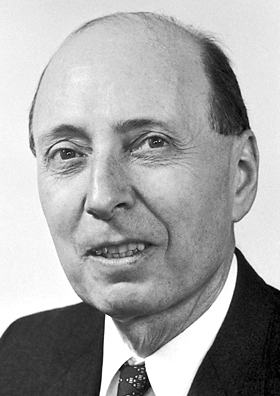
\includegraphics[width=2cm]{Wigner}
   }
   \only<2>{
    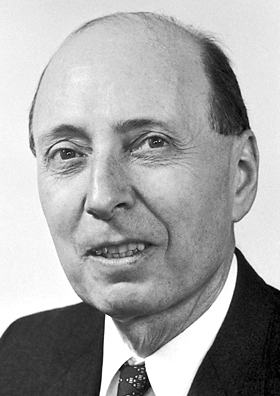
\includegraphics[height=2cm]{Wigner}
   }
   \only<3>{
    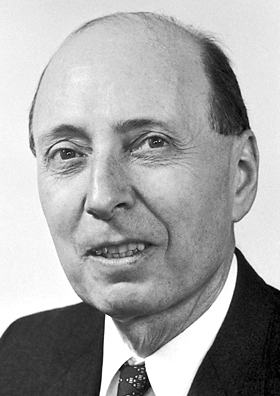
\includegraphics[width=2cm,height=2cm]{Wigner}
   }
   \only<4>{
    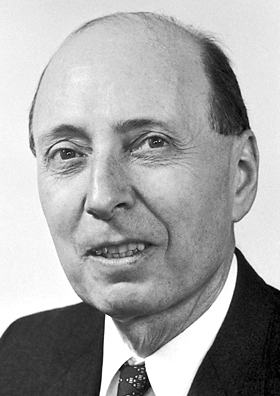
\includegraphics[width=2cm,height=2cm,keepaspectratio]{Wigner}
   }
   \only<5>{
    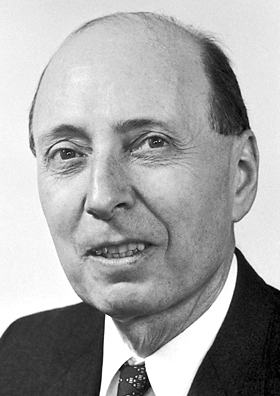
\includegraphics[scale=0.2]{Wigner}
   }
   \only<6>{
    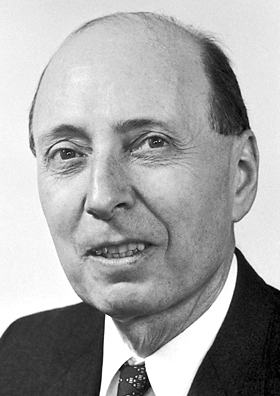
\includegraphics[width=2cm,angle=45]{Wigner}
   }
   \only<7>{
    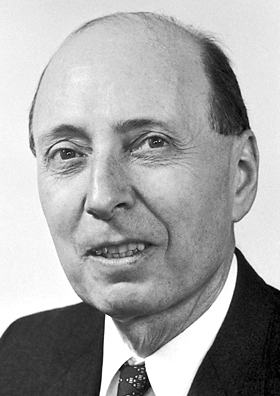
\includegraphics[width=2cm,clip,trim= 2cm 2cm 2cm 2cm]{Wigner}
   }
  \end{column}
 \end{columns}
\end{frame}

\begin{frame}[fragile]{Float-ok}
 \myemph{Hogyan lehet a objektumokat a szövegben elhelyezni?}
 \begin{itemize}
  \item A szövegben közvetlenül megmondjuk, hogy hol lesz
  \item Float-ot készítünk belőle. Ekkor automatikusan lesz
  \begin{itemize}
   \item számozás $\Rightarrow$ Tudunk rá hivatkozni.
   \item kép/táblázat aláírás
   \item és a szövegben elhelyezi az optimális tördelésnek megfelelően
  \end{itemize}
 \end{itemize}
 \vspace*{-20pt}
\begin{lstlisting}
...
% preambulumban:
\usepackage{graphicx}
\usepackage{float}
\begin{ducument}
...
 \begin{figure}[placement specifiers]
  \centering
  \includegraphics[attr1=val1,...]{imagename}
  \caption{Abrafelirat}\label{fig:abracska}
 \end{figure}
...
\end{ducument}
\end{lstlisting}
\end{frame}

\begin{frame}[fragile]{Hasznos csomagok float-ok kezeléséhez}{}
 \begin{itemize}
  \item subfig környezet\footnote{ftp://ctan.tug.org/tex-archive/macros/latex/contrib/subfig/subfig.pdf}: több alképből álló float kezelésére
  \item overpic\footnote{http://www.ctan.org/pkg/overpic}: képekre lehet bármit rátenni vele
  \item minipage: nem kimondottan képek kezelésére, de erre is hasznos
  \item wrapfig: képek köré lehet futtatni szöveget
 \end{itemize}
 
\end{frame}

\section{Saját parancsok definiálása}
\begin{frame}[fragile]{Saját parancsok definiálása}
 Több lehetőségünk is van
 \begin{itemize}
  \item \lstinline|\newcommand|: új parancs definiálásához
  \item \lstinline|\recommand|: már létező parancs újradefiniálásához
  \item \lstinline|\providecommand|: olyan parancs definiálásához, amely még nem létezik
 \end{itemize}
 
 Mindegyik szintaxisa ugyanolyan:
\begin{lstlisting}
\newcommand{\commandname}[num]{definition}
\end{lstlisting}

1. Feladat: írjunk egy macro-t, amellyel mértékegységeket tudunk beírni.

2. Feladat: írjunk egy macro-t, amely készít nekünk kétindexes tenzorokat.
\end{frame}

\begin{frame}[fragile]{Megoldások}
\begin{lstlisting}
\newcommand{\me}[1]{%
\mathrm{#1}%
}
\end{lstlisting}

\begin{lstlisting}
\newcommand{\tensor}[4]{%
^{#1\phantom{#2}#3\phantom{#4}}_{#2\phantom{#1}#4\phantom{#3}}%
}
\end{lstlisting}
\end{frame}

\section{Bibliography használata}

\begin{frame}[fragile]{Bibliography használata}
 Példafájl!
\end{frame}

\section{Nagy példa}

\begin{frame}[fragile]{JK}
 Példafájl!
\end{frame}

\section{Speciális class-ok}

\begin{frame}{Speciális class-ok}
 \begin{itemize}
  \item Prezentációk készítése: pl.\ a beamer class-szal lehetséges\footnote{\url{http://www.tug.org/teTeX/tetex-texmfdist/doc/latex/beamer/beameruserguide.pdf}}
  \item Poszterek készítése: pl.\ a baposter class-szal\footnote{\url{http://www.brian-amberg.de/uni/poster/}}.
  \item Önéletrajz készítése: pl.\ a modern cv class-szal\footnote{\url{http://www.ctan.org/tex-archive/macros/latex/contrib/moderncv}}.
 \end{itemize}
 
 Rengeteg további template és class található a \url{http://www.latextemplates.com/} oldalon. Azért csak óvatosan\dots
\end{frame}




\end{document}